\documentclass[conference]{IEEEtran}
\usepackage{graphicx} % Required for inserting images
\usepackage{amsmath} % Equation

\usepackage{pgfplots}
\usepackage{pgfplotstable}
\usepgfplotslibrary{statistics}
\pgfplotsset{compat=newest}
% \usepackage{filecontents}
\usepgfplotslibrary{fillbetween} % Load the fillbetween library
\usepgfplotslibrary{groupplots}
\usepackage{pgfgantt}

%%% for tables %%%
\usepackage{siunitx}
\usepackage{booktabs}
\usepackage{amsmath,amssymb}

%%% for multi-header table %%%
\usepackage{multirow}
\usepackage{collcell}
\usepackage{colortbl}
\usepackage{xcolor}
\usepackage{datatool}

\pgfplotstableset{%
  every head row/.style={before row=\toprule, after row=\midrule},
  every last row/.style={after row=\bottomrule}
}

\newcommand*\rot{\rotatebox{90}}
\newcommand{\rowhead}[1]{\dorowhead#1\relax}
\def\dorowhead#1#2\relax{$#1_{#2}$}


%%%%%%%%%%%% For one box plot %%%%%%%%%%%%
\pgfplotsset{
    box plot/.style={
        /pgfplots/.cd,
        black, % color
        only marks,
        mark=-,
        mark size=\pgfkeysvalueof{/pgfplots/box plot width},
        /pgfplots/error bars/y dir=plus,
        /pgfplots/error bars/y explicit,
        /pgfplots/table/x index=\pgfkeysvalueof{/pgfplots/box plot x index},
    },
    box plot box/.style={
        /pgfplots/error bars/draw error bar/.code 2 args={%
            \draw  ##1 -- ++(\pgfkeysvalueof{/pgfplots/box plot width},0pt) |- ##2 -- ++(-\pgfkeysvalueof{/pgfplots/box plot width},0pt) |- ##1 -- cycle;
        },
        /pgfplots/table/.cd,
        y index=\pgfkeysvalueof{/pgfplots/box plot box top index},
        y error expr={
            \thisrowno{\pgfkeysvalueof{/pgfplots/box plot box bottom index}}
            - \thisrowno{\pgfkeysvalueof{/pgfplots/box plot box top index}}
        },
        /pgfplots/box plot
    },
    box plot top whisker/.style={
        /pgfplots/error bars/draw error bar/.code 2 args={%
            \pgfkeysgetvalue{/pgfplots/error bars/error mark}%
            {\pgfplotserrorbarsmark}%
            \pgfkeysgetvalue{/pgfplots/error bars/error mark options}%
            {\pgfplotserrorbarsmarkopts}%
            \path ##1 -- ##2;
        },
        /pgfplots/table/.cd,
        y index=\pgfkeysvalueof{/pgfplots/box plot whisker top index},
        y error expr={
            \thisrowno{\pgfkeysvalueof{/pgfplots/box plot box top index}}
            - \thisrowno{\pgfkeysvalueof{/pgfplots/box plot whisker top index}}
        },
        /pgfplots/box plot
    },
    box plot bottom whisker/.style={
        /pgfplots/error bars/draw error bar/.code 2 args={%
            \pgfkeysgetvalue{/pgfplots/error bars/error mark}%
            {\pgfplotserrorbarsmark}%
            \pgfkeysgetvalue{/pgfplots/error bars/error mark options}%
            {\pgfplotserrorbarsmarkopts}%
            \path ##1 -- ##2;
        },
        /pgfplots/table/.cd,
        y index=\pgfkeysvalueof{/pgfplots/box plot whisker bottom index},
        y error expr={
            \thisrowno{\pgfkeysvalueof{/pgfplots/box plot box bottom index}}
            - \thisrowno{\pgfkeysvalueof{/pgfplots/box plot whisker bottom index}}
        },
        /pgfplots/box plot
    },
    box plot median/.style={
        /pgfplots/box plot,
        /pgfplots/table/y index=\pgfkeysvalueof{/pgfplots/box plot median index}
    },
    box plot width/.initial=1em,
    box plot x index/.initial=0,
    box plot median index/.initial=1,
    box plot box top index/.initial=2,
    box plot box bottom index/.initial=3,
    box plot whisker top index/.initial=4,
    box plot whisker bottom index/.initial=5,
}

\newcommand{\boxplot}[2][]{
    \addplot [box plot median,#1] table {#2};
    \addplot [forget plot, box plot box,#1] table {#2};
    \addplot [forget plot, box plot top whisker,#1] table {#2};
    \addplot [forget plot, box plot bottom whisker,#1] table {#2};
}

%%%%%%%%%%%%  For color boxplot %%%%%%%%%%%%
% Nice color sets, see see http://colorbrewer2.org/ 
\usepgfplotslibrary{colorbrewer}
% initialize Set1-4 from colorbrewer (we're comparing 4 classes),
\pgfplotsset{compat = 1.15, 
             cycle list/Set1-8} 
% Tikz is loaded automatically by pgfplots
% \usetikzlibrary{pgfplots.statistics, pgfplots.colorbrewer} 
% provides \pgfplotstabletranspose


%%%%%%%%%%%%  For bar plot %%%%%%%%%%%%

\usetikzlibrary{arrows.meta}

%%%%%%%%%%%%  For secondary y axis plot %%%%%%%%%%%%

% Define the style for the secondary y-axis
\pgfplotsset{
    y2axis style/.style={
        axis y line*=right,
        axis x line=none,
        ylabel= {y2 axis label},
        yticklabel style= {color=red},
        ylabel style= {color=red, align=center},
    }
}


%%%%%%%%%%%%%%%%%%%% Removing the legend 2 bars for bar plot %%%%%%%%%%%%%%%%%%%%%%%
\pgfplotsset{compat=newest,
        /pgfplots/ybar legend/.style={
        /pgfplots/legend image code/.code={%
        %\draw[##1,/tikz/.cd,yshift=-0.25em]
                %(0cm,0cm) rectangle (3pt,0.8em);},
        \draw[##1,/tikz/.cd,bar width=3pt,yshift=-0.2em,bar shift=0pt]
                plot coordinates {(0cm,0.8em)};},
},
}

%%%%%%%%%%%%%%%%%%%% For charts %%%%%%%%%%%%%%%%%%%%
\usepackage{tikz}
\usetikzlibrary{shapes.geometric, arrows}
\usetikzlibrary{positioning, ext.paths.ortho}

%%%%%%%%%%%% EQS
\DeclareMathOperator*{\argminA}{arg\,min} % Jan Hlavacek
\DeclareMathOperator*{\argmaxA}{arg\,max} % Jan Hlavacek
\DeclareMathOperator*{\maxA}{max} % Jan Hlavacek

%%%%%%%%%%%%%%%%%%%% main %%%%%%%%%%%%%%%%%%%%%%%
\title{PGFPlots/TikZ Boilerplate}
\author{JP Talusan}
\date{March 2024}

\begin{document}

\maketitle
% Read the data/testdata2.dat
\begin{figure}
\centering
\begin{tikzpicture}
\begin{axis} [
    box plot width=2mm, 
    height=3in,
    xtick = {1, 2, 3, 4, 5},
    xticklabels = {A, B, C, D, E},
]
% \boxplot [forget plot, red] {testdata.dat}
\boxplot [
    forget plot, black, width=0.40\textwidth,
    % fill,fill opacity=0.5,
    fill=blue!30!white,
    box plot whisker bottom index=1,
    box plot whisker top index=5,
    box plot box bottom index=2,
    box plot box top index=4,
    box plot median index=3
] {data/testdata2.dat}
% Add extra plot
% \addplot [domain=-2:6, thick, cyan] {-x+25+rnd}; \addlegendentry{Some line}
\end{axis}
\end{tikzpicture}
\caption{One Box Plot}
\end{figure}

\begin{figure}
    \centering
\begin{tikzpicture}
    \pgfplotstableread[col sep=comma]{data/data.csv}\csvdata
    % Boxplot groups columns, but we want rows
    \pgfplotstabletranspose\datatransposed{\csvdata} 
    \begin{axis}[
        boxplot/draw direction = y,
        x axis line style = {opacity=1},
        % axis x line* = bottom,
        % axis y line = left,
        enlarge y limits,
        ymajorgrids,
        grid style={line width=.1pt, draw=gray!10},
        xtick = {1, 2, 3, 4},
        xticklabel style = {align=center, font=\small, rotate=60},
        xticklabels = {Apples, Oranges, Bananas, Melons},
        xtick style = {draw=none}, % Hide tick line
        ylabel = {Juiciness},
        % ytick = {20, 40},
        width=0.45\textwidth
    ]
        \foreach \n in {1,...,4} {
            % \addplot+[mark=*, boxplot, fill, draw=black] table[y index=\n] {\datatransposed};
            % \addplot+[mark=*, boxplot, fill, draw=black, opacity=30] table[y index=\n] {\datatransposed};
            \addplot[
                mark=*, 
                boxplot, 
                fill=blue!30, 
                draw=black, 
                opacity=30
            ] table[y index=\n] {\datatransposed};
            
        }
    \end{axis}
\end{tikzpicture}
\caption{Box Plot with Color}
\label{fig:enter-label}
\end{figure}


\begin{figure}
\centering
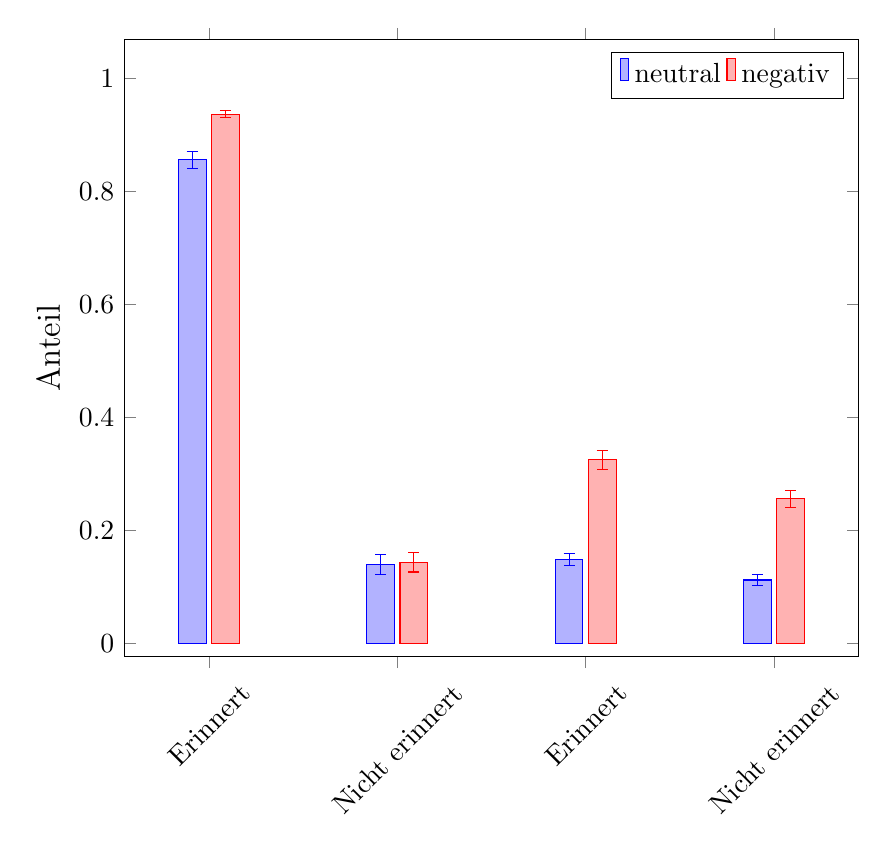
\begin{tikzpicture}
\begin{axis}[
    % instead of scaling
    width=0.9\linewidth,
    ybar,
    enlargelimits=0.15,
    legend style={
    % to save space I would place the legend inside the axis, at least with these data
      %at={(0.5,-0.2)},
      %anchor=north,
      legend columns=-1
    },
    ylabel={Anteil},
    ylabel style={font=\large},
    xtick=data,
    % use explicit ticklabels instead of symbolc x coords
    xticklabels={Erinnert,Nicht erinnert,Erinnert,Nicht erinnert},
    xticklabel style={
    %  text width=2cm,
      % yshift=-18pt, % move xticks down a bit
    %  align=center
    rotate=45
    },
    %%%%%%% extra ticks
    % extra x ticks={1.5,3.5},
    % extra x tick labels={Freie Wiedergabe Tag 1,Freie Wiedergabe Tag 2},
    % extra x tick style={
    %   %%%%%%%% because the xticklabel style also affects the extra ticks, 
    %   %%%%%%%% shift extra ticklabels back up
    %   ticklabel style={yshift=13pt},
    %   %%%%%%%% tickwidth is actually the length of of the ticks (the small lines)
    %   tickwidth=0
    % }
]
%neutral
\addplot[blue,fill=blue!30!white,error bars/.cd,y dir=both,y explicit,]
coordinates{
   (1,0.8560) +-(0.01503,0.01503)
   (2,0.1390) +-(0.01737,0.01737)
   (3,0.1481) +-(0.01067,0.01067)
   (4,0.1119) +-(0.00922,0.00922)
};
%negativ
\addplot[red,fill=red!30!white,error bars/.cd,y dir=both,y explicit,]
coordinates {
  (1,0.9365) +- (0.00587,0.00587)
  (2,0.1435) +- (0.01737,0.01737)
  (3,0.3247) +-(0.01695,0.01695)
  (4,0.2556) +-(0.01524,0.01524)
};
\legend{neutral,negativ}
\end{axis}
\end{tikzpicture}
\caption{Unterschrift A}
\label{GedaechtnisBilder}
\end{figure}

% load the data table ...
\pgfplotstableread[col sep=comma]{data/bar_with_error.csv}{\loadedtable}
    % and store the number of columns in `\NoOfCols'
    % (minus 1 because counting in `\foreach' starts with zero
    \pgfplotstablegetcolsof{\loadedtable}
% load the data table ...
\pgfplotstableread[col sep=comma]{data/bar_with_error2.csv}{\loadedtableB}
    % and store the number of columns in `\NoOfCols'
    % (minus 1 because counting in `\foreach' starts with zero
    \pgfplotstablegetcolsof{\loadedtableB}


\begin{figure}
\centering
\begin{tikzpicture}
\begin{axis}[
    width=0.80\linewidth,
    ybar,
    enlargelimits=0.15,
    % legend style={
    %   legend columns=-1
    % },
    legend pos=outer north east,
    ylabel={Anteil},
    ylabel style={font=\large},
    xtick=data,
    % xticklabels from table={\loadedtable}{Condition}, % Read xticklabels from the CSV file
    xticklabel style={
        rotate=45,
    },
]
%neutral
\addplot[blue,fill=blue!30!white,error bars/.cd,y dir=both,y explicit,] table[
  x expr=\coordindex, % Use index for x values
  y=Mean, % y values from "Mean" column
  col sep=comma,
  y error=Error % Error values from "Error" column
] {\loadedtable};

%negativ
\addplot[red,fill=red!30!white,error bars/.cd,y dir=both,y explicit,] table[
  x expr=\coordindex+0.0, % Offset x values for the second plot
  y=Mean, % y values from "Mean" column
  col sep=comma,
  y error=Error % Error values from "Error" column
] {\loadedtableB};


\legend{neutral,negativ}
\end{axis}
\end{tikzpicture}
\caption{Bar with Errors From File}
\label{GedaechtnisBilderB}
\end{figure}



% load the data table ...
\pgfplotstableread[col sep=comma]{data/bar_data_small.csv}{\loadedtable}
    % and store the number of columns in `\NoOfCols'
    % (minus 1 because counting in `\foreach' starts with zero
    \pgfplotstablegetcolsof{\loadedtable}
    \pgfmathtruncatemacro{\NoOfCols}{\pgfplotsretval-1}

\begin{figure}
\centering
\begin{tikzpicture}
    \begin{axis}[
        % adjust the `width' a bit by keeping the default `height'
        % width=1.2*\axisdefaultwidth,
        % height=\axisdefaultheight,
        width=1.0\linewidth,
        % set appropriate `ymax' value so the `nodes near coords' fit to the plot
        % (adjusting the `ymin' value is just to make it look a little bit better)
        % ymin=1e-1,
        % ymax=1e6,
        % there should be no gap between the bars in one group
        ybar=0pt,
        % use data from the table for the xticklabels
        xtick=data,
        xticklabels from table={\loadedtable}{COUNT},
        % to start the bars from the bottom edge of the plot
        % (otherwise they would start from 10^0
        %  borrowed from <http://tex.stackexchange.com/a/86688/95441)
        % log origin=infty,
        % adjust the size of the bars so they don't overlap
        % (you can play with the numerator to change the gap between the groups)
        % bar width=0.85/\NoOfCols,
        % enlarge the x limits so all of the bars are shown
        % (play with the value to adjust the gap on the sides of the plot)
        enlarge x limits={abs=0.6},
        % and position the legend outside of the plot to not overlap with the data
        % legend pos=outer north east,
        legend style={at={(0.03,0.9)},anchor=west},
        % add `nodes near coords'
        % nodes near coords={
        %     % because internally PGFPlots works with floating point numbers, we
        %     % change them to fixed point numbers
        %     \pgfkeys{
        %         /pgf/fpu=true,
        %         /pgf/fpu/output format=fixed,
        %     }%
        %     % check if numbers are greater than 1000 and if so, divide them by
        %     % 1000 to convert them from ms to s scale
        %     \pgfmathparse{
        %         ifthenelse(
        %             \pgfplotspointmeta < 1000,
        %             \pgfplotspointmeta,
        %             \pgfplotspointmeta/1000
        %         )
        %     }%
        %     % to now decide which of the two cases we have, we compare the
        %     % point meta value, but because `\ifnum' compares integers, we first
        %     % have to convert the fixed number to an integer
        %         \pgfmathtruncatemacro{\Y}{\pgfplotspointmeta}%
        %     \ifnum\Y<1000
        %         \pgfmathprintnumber{\pgfmathresult}\,ms
        %     \else
        %         \pgfmathprintnumber{\pgfmathresult}\,s
        %     \fi
        % },
        % set the style of the `nodes near coords'
        % nodes near coords style={
        %     font=\tiny,
        %     rotate=90,
        %     anchor=west,
        % },
        % as basis for the `nodes near coords' use the raw y values
        % point meta=rawy,
        % Distances between ticks
        xtick distance=2,
    ]
        % add the data rows
        \foreach \i in {1,...,\NoOfCols} {
            \addplot table [
                x expr=\coordindex,
                y index=\i,
                col sep=comma,
            ] {\loadedtable};
                % to automatically add the legend entries first extract the
                % column name and store it in `\colname'
                % (this is an undocumented command so far. I borrowed it from
                %  <http://tex.stackexchange.com/q/171021/95441>)
                    \pgfplotstablegetcolumnnamebyindex{\i}\of{\loadedtable}\to{\colname}
                % now you can add the legend entry
                % (because we are in a loop we have to use the "expanded" version)
                \addlegendentryexpanded{\colname};
        }
    \end{axis}
\end{tikzpicture}
\caption{Bar Plot From CSV}
\end{figure}

\pgfplotstableread[col sep=comma]{data/line_plot.csv}{\loadedtable}
    % and store the number of columns in `\NoOfCols'
    % (minus 1 because counting in `\foreach' starts with zero
    \pgfplotstablegetcolsof{\loadedtable}
    % \pgfmathtruncatemacro{\NoOfCols}{\pgfplotsretval-1}

\begin{figure}[htbp]
\centering
\begin{tikzpicture}
\begin{axis}[
    xlabel={Day of the Month},
    ylabel={Value},
    xmin=1, xmax=31, % Adjust the x-axis range to fit the number of days in the month
    ymin=0, % Adjust the y-axis range as needed
    grid=both,
    grid style={line width=.1pt, draw=gray!10},
    major grid style={line width=.2pt,draw=gray!50},
    % minor tick num=4,
    enlarge x limits=false,
    enlarge y limits={upper,value=0.1},
    legend pos=north east,
    width=0.45\textwidth,
    % Adjust steps
    xtick distance=2
]

% Plot the line
\addplot+[no marks, thick, color=red!100] table[x=Day, y=Value, col sep=comma]{\loadedtable};
\legend{Value}


\addplot+[mark=*, thick] table[x=Day, y=Value2, col sep=comma]{\loadedtable};
\legend{Value2}


\end{axis}
\end{tikzpicture}
\caption{Line plot of values over the days of the month}
\end{figure}

\pgfplotstableread[col sep=comma]{data/ypred_vs_ytrue.csv}{\loadedtable}
    % and store the number of columns in `\NoOfCols'
    % (minus 1 because counting in `\foreach' starts with zero
    \pgfplotstablegetcolsof{\loadedtable}
    % \pgfmathtruncatemacro{\NoOfCols}{\pgfplotsretval-1}
    
\begin{figure}[htbp]
\centering
\begin{tikzpicture}
\begin{axis}[
    xlabel={Predicted},
    ylabel={Actual},
    % axis equal image, % Ensure the aspect ratio is 1:1
    grid=both,
    grid style={line width=.1pt, draw=gray!10},
    major grid style={line width=.2pt,draw=gray!50},
    legend pos=north west,
    width=0.9\linewidth,
]

% Add the dashed diagonal line
\addplot+[domain=0:100, dashed, no marks, samples=2] {x}; % Adjust domain as needed
\addlegendentry{Ideal}

% Add the scatter plot
\addplot+[only marks, mark=*, mark options={scale=1}, opacity=0.5] table[x=predicted, y=actual, col sep=comma] {\loadedtable};
\addlegendentry{Predicted vs Actual}

\end{axis}
\end{tikzpicture}
\caption{Comparison of Predicted vs Actual Results}
\end{figure}

% Don't know how to read form file.
\begin{figure}
    \centering
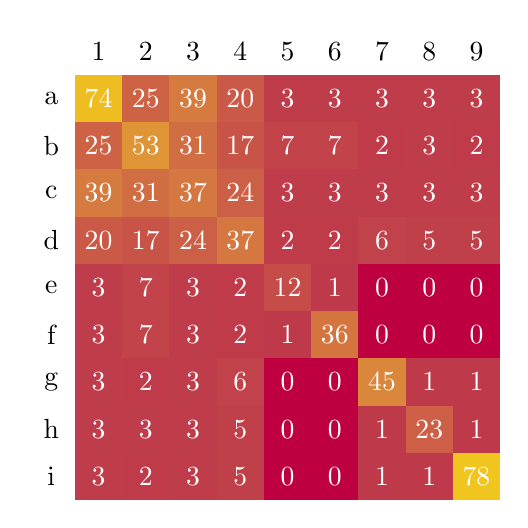
\begin{tikzpicture}[scale=0.6, style={node contents={}}]
  \foreach \y [count=\n] in {
      {74,25,39,20,3,3,3,3,3},
      {25,53,31,17,7,7,2,3,2},
      {39,31,37,24,3,3,3,3,3},
      {20,17,24,37,2,2,6,5,5},
      {3,7,3,2,12,1,0,0,0},
      {3,7,3,2,1,36,0,0,0},
      {3,2,3,6,0,0,45,1,1},
      {3,3,3,5,0,0,1,23,1},
      {3,2,3,5,0,0,1,1,78},
    } {
      % column labels
      \ifnum\n<10
        \node[minimum size=6mm] at (\n, 0) {\n};
      \fi
      % heatmap tiles
      \foreach \x [count=\m] in \y {
        \node[fill=yellow!\x!purple, minimum size=6mm, text=white] at (\m,-\n) {\x};
      }
    }

  % row labels
  \foreach \a [count=\i] in {a,b,c,d,e,f,g,h,i} {
    \node[minimum size=6mm] at (0,-\i) {\a};
  }
\end{tikzpicture}
    % \includegraphics{}
    \caption{Heatmap}
    \label{fig:heatmap}
\end{figure}

\pgfplotstableread[col sep=comma]{data/twobar.csv}\csvdata
% Boxplot groups columns, but we want rows
\pgfplotstabletranspose\datatransposed{\csvdata} 
\pgfplotstablegetcolsof{\datatransposed}
\pgfmathtruncatemacro{\NoOfCols}{\pgfplotsretval-1}
    
\begin{figure}
\centering
\begin{tikzpicture}
\begin{axis}[
boxplot/draw direction=y,
ylabel={segmentation time (secs)},
% height=8cm,
boxplot={
    %
    % Idea: 
    %  place the 
    %  group 1 at 0.3333 and 0.6666
    %  group 2 at 1.3333 and 1.6666
    %  group 3 at 2.3333 and 2.6666
    %  ...
    % in a formular:
    draw position={1/3 + floor(\plotnumofactualtype/2) + 1/3*mod(\plotnumofactualtype,2)},
    %
    % that means the box extend must be at most 0.33333 :
    box extend=0.3,
},
% ... it also means that 1 unit in x controls the width:
% x=2cm,
% ... and it means that we should describe intervals:
xtick={0,1,2,...,10},
x tick label as interval,
xticklabels={%
    {Data set 1\\{\tiny off/on}},%
    {Data set 2\\{\tiny off/on}},%
    {Data set 3\\{\tiny off/on}},%
    {Data set 4\\{\tiny off/on}},%
},
    x tick label style={
        text width=2.5cm,
        align=center
    },
    % Add to cycle for each other boxplot you want to be in a group
    cycle list={{fill=red!30},{fill=blue!30}},
    width=0.45\textwidth
]


\foreach \n in {1,...,\NoOfCols} {
    % \addplot+[mark=*, boxplot, fill, draw=black] table[y index=\n] {\datatransposed};
    % \addplot+[mark=*, boxplot, fill, draw=black, opacity=30] table[y index=\n] {\datatransposed};
    \addplot table[mark=*, y index=\n] {\datatransposed};
    
}

% \addplot
% table[row sep=\\,y index=0] {
% data\\
% 60\\
% 516\\
% 710\\
% 503\\
% 1253\\
% 0\\
% };
% \addplot
% table[row sep=\\,y index=0] {
% data\\
% 759\\
% 419\\
% 309\\
% 883\\
% 299\\
% };

% \addplot
% table[row sep=\\,y index=0] {
% data\\
% 516\\
% 480\\
% 1356\\
% 200\\
% 736\\
% };
% \addplot
% table[row sep=\\,y index=0] {
% data\\
% 684\\
% 340\\
% 700\\
% 325\\
% 377\\
% };

% \addplot
% table[row sep=\\,y index=0] {
% data\\
% 956\\
% 320\\
% 811\\
% 330\\
% 381\\
% };
% \addplot
% table[row sep=\\,y index=0] {
% data\\
% 280\\
% 749\\
% 392\\
% 870\\
% 488\\
% };

% \addplot
% table[row sep=\\,y index=0] {
% data\\
% 658\\
% 579\\
% 891\\
% 545\\
% 558\\
% };
% \addplot
% table[row sep=\\,y index=0] {
% data\\
% 514\\
% 630\\
% 416\\
% 559\\
% 462\\
% };

\end{axis}
\end{tikzpicture}
\caption{Multiple box plots}
\end{figure}

% https://tikz.dev/pgfplots/reference-markers
\begin{figure*}[t]
\centering
\begin{tikzpicture}
\begin{groupplot}[
    group style={
        group size=3 by 1, % 1 column, 3 rows
        % vertical sep=2cm, % Separation between plots
        horizontal sep=2cm, % Separation between plots
    },
    % Divide by the number of plots
    width=0.32\textwidth,
    height=5cm,
]

% First subplot
\nextgroupplot[title=Plot 1, xlabel={X axis 1}, ylabel={Y axis 1}]
\addplot 
[thick, mark=*, mark options={solid, color=blue!30}, color=blue!30]
table[col sep=comma, x=X, y=Y1] {data/multi_plot.csv};

% Second subplot
\nextgroupplot[title=Plot 2, xlabel={X axis 2}, ylabel={Y axis 2}]
\addplot
[mark=oplus]
table[col sep=comma, x=X, y=Y2] {data/multi_plot.csv};

% Third subplot
\nextgroupplot[title=Plot 3, xlabel={X axis 3}, ylabel={Y axis 3}]
\addplot 
[mark=square*, loosely dashed]
table[col sep=comma, x=X, y=Y3] {data/multi_plot.csv};

\end{groupplot}
\end{tikzpicture}
\caption{Multiple subplots columns}
\end{figure*}


%%%%%% MULTI ROWS %%%%%%%
\begin{figure}[t]
\centering
\begin{tikzpicture}
\begin{groupplot}[
    group style={
        group size=1 by 3, % 1 column, 3 rows
        vertical sep=1cm, % Separation between plots
        % horizontal sep=2cm, % Separation between plots
    },
    % Divide by the page width
    width=0.49\textwidth,
    height=5cm,
]

% First subplot
\nextgroupplot[
    title=Plot 1, 
    % xlabel={X axis 1}, 
    ylabel={Y axis 1}
]
\addplot table[col sep=comma, x=X, y=Y1] {data/multi_plot.csv};

% Second subplot
\nextgroupplot[
    title=Plot 2, 
    % xlabel={X axis 2}, 
    ylabel={Y axis 2}
]
\addplot table[col sep=comma, x=X, y=Y2] {data/multi_plot.csv};

% Third subplot
\nextgroupplot[
    title=Plot 3,
    xlabel={X axis 3},
    ylabel={Y axis 3}
]
\addplot
[thick, mark=*, mark options={solid, color=blue!30}, color=blue!30] 
table[col sep=comma, x=X, y=Y3] {data/multi_plot.csv};

\end{groupplot}
\end{tikzpicture}
\caption{Multiple subplots rows}
\end{figure}


%%%%%% 2D %%%%%

\begin{figure}[t]
\centering
\begin{tikzpicture}
\begin{groupplot}[
    group style={
        group size=3 by 2, % 3 column, 2 rows
        vertical sep=0.2cm, % Separation between plots
        horizontal sep=0.2cm, % Separation between plots
    },
    % Divide by the page width
    width=0.45\linewidth,
    height=0.33\textwidth,
]

% First subplot
\nextgroupplot[
    % title=Plot 1, 
    % xlabel={X axis 1}, 
    ylabel={Y axis 1},
    xticklabels={}
]
\addplot table[col sep=comma, x=X, y=Y1] {data/multi_plot.csv};

% Second subplot
\nextgroupplot[
    title=Overall, 
    % xlabel={X axis 2}, 
    % ylabel={Y axis 2}
    yticklabels={},
    xticklabels={}
]
\addplot[thick, mark=*, mark options={solid, color=blue!30}, color=blue!30] table[col sep=comma, x=X, y=Y2] {data/multi_plot.csv};

% Third subplot
\nextgroupplot[
    % title=Plot 3,
    % xlabel={X axis 3},
    % ylabel={Y axis 3}
    yticklabels={},
    xticklabels={}
]
\addplot table[col sep=comma, x=X, y=Y3] {data/multi_plot.csv};

% Fourth subplot
\nextgroupplot[
    % title=Plot 1, 
    xlabel={X axis 1}, 
    ylabel={Y axis 1},
]
\addplot table[col sep=comma, x=X, y=Y4] {data/multi_plot.csv};

% Fifth subplot
\nextgroupplot[
    % title=Plot 2, 
    xlabel={X axis 2}, 
    % ylabel={Y axis 2}
    yticklabels={}
]
\addplot table[col sep=comma, x=X, y=Y5] {data/multi_plot.csv};

% Sixth subplot
\nextgroupplot[
    % title=Plot 3,
    xlabel={X axis 3},
    % ylabel={Y axis 3}
    yticklabels={}
]
\addplot table[col sep=comma, x=X, y=Y6] {data/multi_plot.csv};

\end{groupplot}
\end{tikzpicture}
\caption{Multiple subplots 2D}
\end{figure}


% When Axis labels don't match along the axis because of differences in the ticks:
% 
% \pgfplotsset{compat=1.6, ylabsh/.style={every axis y label/.style={at={(0,0.5)}, xshift=#1, rotate=90}}}  

% Usage:
% \begin{groupplot}[
%     group style={
%         group size=1 by 3, % 1 column, 3 rows
%         vertical sep=0.2cm, % Separation between plots
%         % horizontal sep=2cm, % Separation between plots
%     },
%     ylabsh=-2.5em,
% ]

% \end{groupplot}


% Read the data from the csv file
% \pgfplotstableread[col sep=comma]{data/bar_with_error.csv}{\loadedtable}
\pgfplotstableread[col sep=comma]{data/secondary_y.csv}\datatable

% Legend option will be in the secondary y axis

% Creating arguments
\newcommand\axisheight{8cm}

\begin{figure}
    \centering
\begin{tikzpicture}
\begin{axis}[
    width=0.45\textwidth,
    height=\axisheight,
    xlabel={$x$},
    ylabel={$y1$},
    ylabel style={rotate=-90},
    tick pos=left
]

% Plot the data for y1
\addplot [blue, mark=*] table [x=x, y={y1}] {\datatable};
% Add a label to the first axis and use that later to add the legends.
\label{firstYplot}
% \addlegendentry{$y1$}

% Done with the first axis
\end{axis}

% Now, add the secondary axis with the `y2axis style` defined earlier
\begin{axis}[
    width=0.45\textwidth,
    height=\axisheight,
    axis x line=none,
    axis y line*=right,
    ylabel={$y2$},
    yticklabel style={color=red},
    ylabel style={rotate=-90, color=red},
    % xmin=0,
    % xmax=10,
    ymin=0,
    ymax=10,
    legend style={at={(0.22, 0.88)}, anchor=south},
    % Legend option is here.
    legend columns=-1,    
]

% Adding the legend by referencing the first plot within the Secondary axis.
\addlegendimage{/pgfplots/refstyle=firstYplot}\addlegendentry{$H$}
% Plot the data for y2 using a secondary axis on the right
% \addplot [red, mark=square] table [x={x}, y={y2}] {\datatable};
\addplot [red, mark=square] table [x={x}, y={y2}] {\datatable};
\addlegendentry{$y^2$}

% Done with the second axis
\end{axis}
\end{tikzpicture}

    \caption{Secondary Y-Axis}
    \label{fig:y-axis}
\end{figure}

\pgfplotstableread[col sep=comma]{data/multi_plot.csv}{\data}

% \pgfplotstableread{
% T   A   B   C
% 20  0   450 43
% 23  0   400 42
% 25  0   350 41
% 30  0   320 40
% 40  0   300 40
% 20  10  400 38
% 23  10  380 37
% 25  10  350 36
% 30  10  310 35
% 40  10  280 40
% }\data

% \pgfplotstablesort[sort key={T}]{\sorted}{\data}

   % \pgfplotstabletypeset[row predicate/.code={%
   % \pgfplotstablegetelem{#1}{T}\of{\sorted}
   % \ifnum\pgfplotsretval=20\relax
   % \else\pgfplotstableuserowfalse\fi}]
   % {\sorted}

\begin{figure}
   \begin{tikzpicture}
    \begin{axis}[
     xlabel=X,
     ylabel=Y1,
     % Grids
    minor x tick num=5,
    minor y tick num=5,
    grid=both,
    ymajorgrids=true,
    yminorgrids=true,
    % xmajorgrids=false,
    xminorgrids=false,
    major grid style={line width=.2pt,draw=gray!30},
    %
    x filter/.code={\pgfplotstablegetelem{\coordindex}{Y2}\of{\data}
                    \ifnum\pgfplotsretval>14
                    \else
                    \def\pgfmathresult{}
                    \fi
                   },
    ]
   \addplot[only marks] table[x=X,y=Y1] {\data};
   \end{axis}
   \end{tikzpicture}
   \caption{Filtering a csv and adding major and minor grids}
\end{figure}

% multiple restricting commands
\pgfplotstableread[col sep=comma]{data/restricted_data.csv}\alldata


\begin{figure}
\centering
\begin{tikzpicture}

% Read the data from the csv file
% \pgfplotstableread[col sep=comma]{data/bar_with_error.csv}{\loadedtable}
\begin{axis}[
    width=0.52\textwidth,
    % height=\axisheight,
    % xlabel={Days},
    % xtick = {1, 2, 3, 4, 5, 6, 7, 8, 9, 10},
    % ylabel={Energy (kWh)},
    ylabel style={rotate=0},
    % tick pos=left,
    cycle list name=color list,
    % legend columns=4,
    % legend style={at={(1.0, 1.01)}, anchor=south},
    % group style={
    %     group size=2 by 2, % 1 column, 3 rows
    %     vertical sep=1.0cm, % Separation between plots
    %     horizontal sep=0.8cm, % Separation between plots
    % },
    % Filtering
    % x filter/.code={\pgfplotstablegetelem{\coordindex}{month}\of{\alldata}
    %             \ifnum\pgfplotsretval=6
    %             \else
    %             \def\pgfmathresult{}
    %             \fi
    %            },
]

%  Will only plot data with policy == 0
\addplot [blue!80, mark=o] 
         table [
            x=day, 
            y={need}, 
            meta=policy,
            restrict expr to domain={\thisrow{policy}}{0:0},
            restrict expr to domain={\thisrow{month}}{6:6}
          ] {\alldata};
\addlegendentry{Restrict 0 and 6}
          
\addplot [red!80, mark=square*] 
         table [
            x=day, 
            y={need}, 
            meta=policy,
            restrict expr to domain={\thisrow{policy}}{1:1},
            restrict expr to domain={\thisrow{month}}{11:11}
          ] {\alldata};
\addlegendentry{Restrict 1 and 11}


\end{axis}
\end{tikzpicture}
\caption{Restricting based on multiple row value}
\end{figure}

\pgfplotstableread[col sep=comma]{data/fig_1_to_jp_r_3.csv}{\routethree}

\begin{figure}[htbp]
\centering
\begin{tikzpicture}
\begin{axis}[
    xlabel={Trip Load},
    ylabel={Number of\\Trips},
    % xmin=1, xmax=31, % Adjust the x-axis range to fit the number of days in the month
    ymin=0, % Adjust the y-axis range as needed
    grid=both,
    grid style={line width=.1pt, draw=gray!10},
    major grid style={line width=.2pt,draw=gray!50},
    % minor tick num=4,
    enlarge x limits=false,
    enlarge y limits={upper,value=0.1},
    legend pos=north east,
    width=0.45\textwidth,
    height=2in,
    % Adjust steps
    % xtick distance=2
    % Changing label format 1:
    % /pgf/number format/.cd,
    %         use comma,
    %         1000 sep={}
    % Changing label format 2:
    scaled y ticks=base 10:-3,
    ytick scale label code/.code={},
    yticklabel={\pgfmathprintnumber{\tick}k},
    % NEeded to new line the label
    ylabel style={align=center}
]

% Create a named path for the horizontal axis.
% https://www.sqlpac.com/en/documents/latex-pgfplots-tikz-filling-areas-under-and-between-curves.html
\path [name path=xaxis]
      (\pgfkeysvalueof{/pgfplots/xmin},0) --
      (\pgfkeysvalueof{/pgfplots/xmax},0);
      
% Plot the line
\addplot[blue, name path=a, no markers, smooth, thick] table[x=trip_load, y=transit_date, col sep=comma]{\routethree};
\legend{Route 3}

\addplot+[blue!30, opacity=0.4] fill between [of=a and xaxis, soft clip={domain=-1:10}];
% \legend{Value2}


\end{axis}
\end{tikzpicture}
\caption{Adding Fill between}
\label{fig:heavy_tail}
\end{figure}

\begin{figure}
    \centering
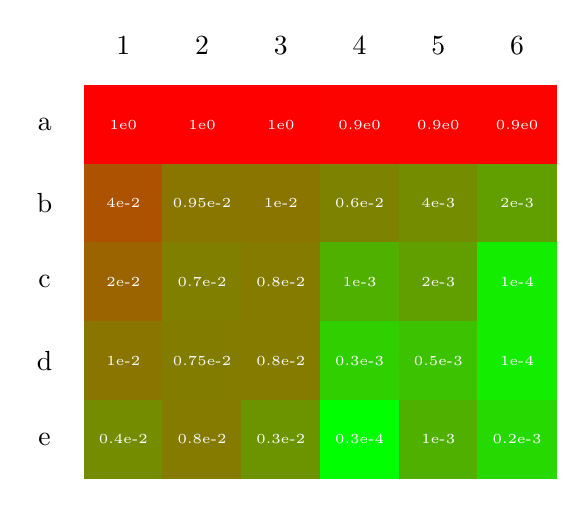
\begin{tikzpicture}
\foreach \y [count=\n] in {
{1e0, 1e0, 1e0, 0.9e0, 0.9e0, 0.9e0},
{4e-2, 0.95e-2, 1e-2, 0.6e-2, 4e-3, 2e-3},
{2e-2, 0.7e-2, 0.8e-2, 1e-3, 2e-3, 1e-4},
{1e-2, 0.75e-2, 0.8e-2, 0.3e-3, 0.5e-3, 1e-4},
{0.4e-2, 0.8e-2, 0.3e-2 ,0.3e-4, 1e-3, 0.2e-3},
} {
\node at (\n, 0) {\n};
\foreach \x [evaluate=\x as \shade using -10*ln(\x), count=\m] in \y {
\node[
fill=green!\shade!red,
minimum size=10.1mm,
text=white, font=\tiny] at (\m,-\n) {\x};
}}
\foreach \a [count=\i] in {a,b,c,d,e} {
\node at (0,-\i) {\a};
}
\end{tikzpicture}
    \caption{Caption}
    \label{fig:enter-label}
\end{figure}

% https://tex.stackexchange.com/questions/102385/how-to-draw-a-return-arrow-from-node-3-to-node-1
% https://tex.stackexchange.com/questions/539468/how-to-define-a-maximum-height-for-a-tikz-decision-node
% https://www.overleaf.com/learn/latex/LaTeX_Graphics_using_TikZ%3A_A_Tutorial_for_Beginners_(Part_3)%E2%80%94Creating_Flowcharts
\newcommand\nodebg{white!100}

\tikzstyle{startstop} = [rectangle, rounded corners, minimum width=3cm, minimum height=1cm,text centered, draw=black, fill=\nodebg, text width=3cm]

\tikzstyle{io} = [trapezium, trapezium left angle=70, trapezium right angle=110, minimum width=3cm, minimum height=1cm, text centered, draw=black, fill=\nodebg]

\tikzstyle{process} = [rectangle, minimum width=3cm, minimum height=1cm, text centered, text width=3cm, draw=black, fill=\nodebg]

\tikzstyle{decision} = [diamond, minimum width=3cm, minimum height=1cm, text centered, draw=black, fill=\nodebg, text width=2cm, aspect=1.4]

\tikzstyle{arrow} = [thick,->,>=stealth]

\tikzset{
  block/.style={rectangle,draw,minimum size=1cm},
  line/.style={draw, -latex},
}

\begin{figure}
% \centering
\begin{tikzpicture}[node distance=0.5cm, 
  scale=0.8, transform shape,
  % auto,
  /utils/temp/.style={#1/.style={to path={r-#1(\tikztotarget)\tikztonodes}}},
  /utils/temp/.list={ud, rl, du, lr}
  ]
\node (start) [startstop] {\texttt{execute()}};
\node (dec1) [decision, below=of start] {EventQueue Empty?};

\node (pro1) [process, right=of dec1] {Simulation finished};
\node (pro2) [process, below=of dec1] {Execute all events in current timestep};
\node (pro3) [process, below=of pro2] {Update environment and state};

\node (dec2) [decision, below=of pro3] {Did cars arrive?};
\node (pro4) [process, right=of dec2] {Assign cars to chargers};
\node (pro5) [process, below=of dec2] {Get charger actions from policy};
\node (pro6) [process, below=of pro5] {Take policy action and update state};

\node (pro7) [process, below=of pro6] {Log state and actions};
\node (pro8) [process, below=of pro7] {Increment timestep};


\draw [arrow] (start) -- (dec1);
\draw [arrow] (dec1) -- node[anchor=south] {yes} (pro1);
\draw [arrow] (dec1) -- node[anchor=east] {no} (pro2);
\draw [arrow] (pro2) -- (pro3);
\draw [arrow] (pro3) -- (dec2);
\draw [arrow] (dec2) -- node[anchor=south] {yes} (pro4);
\draw [arrow] (dec2) -- node[anchor=east] {no} (pro5);
\draw [arrow] (pro4) |- (pro5);

\draw [arrow] (pro5) -- (pro6);
\draw [arrow] (pro6) -- (pro7);
\draw [arrow] (pro7) -- (pro8);
\path [line] (pro8) edge[lr] (start);

% \draw [arrow] (pro8) -- (start);


% \draw [arrow] (start) -- (in1);
% \draw [arrow] (in1) -- (pro1);
% \draw [arrow] (pro1) -- (dec1);
% \draw [arrow] (dec1) -- (pro2a);
% \draw [arrow] (dec1) -- (pro2b);

% \draw [arrow] (dec1) -- node[anchor=east] {yes} (pro2a);
% \draw [arrow] (dec1) -- node[anchor=south] {no} (pro2b);

% \draw [arrow] (pro2a) -- (out1);
% \draw [arrow] (out1) -- (stop);
% \draw [arrow] (pro2b) |- (pro1);

\end{tikzpicture}
\caption{Chart drawn using TikZ}
\end{figure}

\begin{figure*}
    \centering
    
\begin{ganttchart}[
y unit title=0.3cm,
y unit chart=0.4cm,
x unit=0.5cm,
vgrid,hgrid, 
title label anchor/.style={below=-1.6ex},
title left shift=.05,
title right shift=-.05,
title height=1.4,
progress label text={},
bar height=0.7,
group right shift=0,
group top shift=.4,
group height=.4]{1}{24}
%labels
\gantttitle{Months}{24} \\
\gantttitle{1}{2} 
\gantttitle{2}{2} 
\gantttitle{3}{2} 
\gantttitle{4}{2} 
\gantttitle{5}{2} 
\gantttitle{6}{2} 
\gantttitle{7}{2} 
\gantttitle{8}{2} 
\gantttitle{9}{2} 
\gantttitle{10}{2} 
\gantttitle{11}{2} 
\gantttitle{12}{2} \\
%tasks
\ganttbar{Task 1.1}{1}{2} \\
\ganttbar{Task 1.2}{3}{4} \\
\ganttbar{Task 1.3}{4}{7} \\
\\
\ganttbar{Task 2.1}{3}{4} \\
\ganttbar{Task 2.2}{5}{6} \\
\ganttbar{Task 2.3}{7}{10} \\
\ganttbar{Task 2.4}{9}{16} \\
\ganttbar{Task 2.5}{9}{16} \\
\\
\ganttbar{Task 3.1}{11}{14} \\
\ganttbar{Task 3.2}{15}{18} \\
\\
\ganttbar{Task 4.1}{1}{2} \\
\ganttbar{Task 4.2}{17}{21} \\
\ganttbar{Task 4.3}{21}{24} \\
\\
\ganttbar{Task 5.1}{23}{24} \\
\ganttbar{Task 5.2}{23}{24} \\
% \ganttbar{task 4}{11}{15} \\
% \ganttbar[progress=33]{task 5}{20}{22} \\
% \ganttbar{task 6}{18}{19} \\
% \ganttbar{task 7}{16}{18} \\
% \ganttbar[progress=0]{task 8}{21}{24}

%relations 
\ganttlink{elem2}{elem5} 
\ganttlink{elem2}{elem6} 
\ganttlink{elem2}{elem7} 
\ganttlink{elem7}{elem11} 
% \ganttlink{elem3}{elem4} 
% \ganttlink{elem1}{elem5} 
% \ganttlink{elem3}{elem5} 
% \ganttlink{elem2}{elem6} 
% \ganttlink{elem3}{elem6} 
% \ganttlink{elem5}{elem7} 
\end{ganttchart}


    \caption{Caption}
    \label{fig:gantt}
\end{figure*}


\begin{equation}
    % \sum_{s' \in \mathcal{S}} \sum_{r \in \mathcal{R}} p (s', r| s, a) = 1, \text{for all  } s \in \mathcal{S}, a \in \mathcal{A} (s)
    % \mathcal{S} \times \mathcal{S} \times \mathcal{A} \rightarrow [0, 1]
    % \pi^*(s) = \argmaxA_{\pi} \mathcal{U}^{\pi}(s)
    % U^{\pi}_{k+1} (s) = R(s, \pi(s)) + \gamma \sum_{s'} T(s'|s,\pi(s)) U^{\pi}_{k} (s')
    % U(s) = \maxA_{a} Q(s, a)
    % \pi(s) = \argmaxA_{a} Q(s, a)
    \mathcal{O}(|\mathcal{S}| \times |\mathcal{A}|)
\end{equation}


% % load the data table ...
\pgfplotstableread[col sep=comma]{data/rishav.csv}{\loadedtable}
    % and store the number of columns in `\NoOfCols'
    % (minus 1 because counting in `\foreach' starts with zero
    % \pgfplotstablegetcolsof{\loadedtable}


\begin{figure*}
\centering
\begin{tikzpicture}
\begin{axis}[
    width=0.9\linewidth,
    height=2in,
    ybar,
    legend style={at={(0.3, 1.01)}, anchor=south},
    legend columns = -1,
    ylabel={Cost {\$}},
    ylabel style={font=\large},
    xlabel style={font=\small},
    xtick={0, 1, 2, 3, 4, 5, 6},
    xticklabels from table={\loadedtable}{policy}, % Read xticklabels from the CSV file
    tick pos=left,
    minor x tick num=5,
    minor y tick num=5,
    grid=both,
    ymajorgrids=true,
    yminorgrids=true,
    % xmajorgrids=false,
    xminorgrids=false,
    major grid style={line width=.2pt,draw=gray!30},
]
%neutral
\addplot[blue,fill=blue!50!white,  area legend,error bars/.cd,y dir=both,y explicit,] table[
  x expr=\coordindex, % Use index for x values
  y=demand_charge_mean, % y values from "Mean" column
  col sep=comma,
  y error=demand_charge_std % Error values from "Error" column
] {\loadedtable};
\label{firstYplot}

\addplot[red,fill=red!40!white, area legend, error bars/.cd,y dir=both,y explicit,] table[
  x expr=\coordindex, % Use index for x values
  y=energy_cost_mean, % y values from "Mean" column
  col sep=comma,
  y error=energy_cost_std % Error values from "Error" column
] {\loadedtable};
\legend{Demand cost (\$), Energy cost(\$)}

\end{axis}

\begin{axis}[
    width=0.9\linewidth,
    height=2in,
    axis x line=none,
    axis y line*=right,
    % enlarge x limits=0.25,
    % ybar,
    legend style={at={(0.8, 1.01)}, anchor=south},
    legend columns = -1,
    ylabel={SoC Gap (kWh)},
    ylabel style={font=\large},
    xtick={0, 1, 2, 3, 4, 5, 6},
    xticklabels from table={\loadedtable}{policy}, % Read xticklabels from the CSV file
    ymin=-10,
    ymax=50,
    % scaled y ticks = false,
]
% \addlegendimage{/pgfplots/refstyle=firstYplot}\addlegendentry{demand charge, energy cost}
\addplot[black!100,error bars/.cd,y dir=both,y explicit,] table[
  x expr=\coordindex+1.0, % Use index for x values
  y=soc_diff_mean, % y values from "Mean" column
  col sep=comma,
  y error=soc_diff_std % Error values from "Error" column
] {\loadedtable};
% \addplot[black,dashed,domain = 1:6,samples = 2] {0};
\legend{Energy Gap (kWh)}

\end{axis}
\end{tikzpicture}
\caption{Comparison of demand cost and energy cost against SoC difference across different policies. A positive SoC Gap means that the cars departed with more charge than required. If it's negative, they departed with less charge than required. Ideally SoC gap should be 0.}
\label{fig:cost_comp}
\vspace{-5mm}
\end{figure*}




\begin{filecontents}{testdata.csv}
theta, x, y
, jp, test
30.0,   0.0,    0.0
60.0,   1.9098, 5.8779
90.0,   6.9098, 9.5106
120.0,  13.09,  9.5106
150.0,  18.09,  5.8779
180.0,  20.0,   0.0
\end{filecontents}

\pgfplotstableread[col sep=comma]{testdata.csv}{\table}

\begin{table*}
\centering
\caption{Reading Table from a File with \textbf{siunitx}.}
\pgfplotstabletypeset[
    % dec sep align=S,    % Use the siunitx `S` column type for aligning at decimal point
    fixed,fixed zerofill,     % Fill numbers with zeros
    precision=3,        % Set number of decimals
    display columns/0/.style={
        precision=1,    % Change for first column (column index 0)
        column name=$\theta_{2,i}$
    },
    % display columns/1/.style={column name=$X$,column type={S}},
    % display columns/2/.style={column name=$Y$,column type={S}},
    every row 0 column 1/.style={string type},
    every row 0 column 2/.style={string type},
    every head row/.style={before row=\toprule, after row=\midrule},
    every last row/.style={after row=\bottomrule},
  every row 2 column 1/.style={
    postproc cell content/.style={
      @cell content/.add={$\bf}{$}
    }
  },
    ] {\table}
\label{table:read_csv}
\end{table*}


\begin{filecontents*}[overwrite]{table_data.csv}
Metric,PSM_F1,PSM_P,PSM_R,SMD_F1,SMD_P,SMD_R,SWAT_F1,SWAT_P,SWAT_R,WADI_F1,WADI_P,WADI_R
OCSVM,0.347,0.718,0.236,0.185,0.894,0.589,0.904,0.417,0.635,0.722,0.859,0.113
IF,0.762,0.812,0.471,0.308,0.978,0.643,0.213,0.983,0.500,0.789,0.226,0.925
LOF,0.163,0.299,0.576,0.873,0.034,0.441,0.722,0.119,0.387,0.617,0.935,0.651
AnomalyTransformer,0.742,0.198,0.801,0.520,0.631,0.484,0.998,0.776,0.125,0.813,0.277,0.439
ImDiffusion,0.467,0.665,0.227,0.849,0.115,0.308,0.489,0.657,0.816,0.372,0.738,0.201
GANF,0.558,0.971,0.429,0.175,0.919,0.760,0.682,0.304,0.206,0.098,0.837,0.950
MTGFlow,0.214,0.571,0.663,0.724,0.046,0.926,0.367,0.855,0.740,0.961,0.483,0.592
WENFLOW (Ours),0.899,0.325,0.917,0.634,0.550,0.197,0.760,0.802,0.415,0.883,0.1,0.270
\end{filecontents*}

\sisetup{
detect-weight=true,
detect-inline-weight=math,
round-mode      = places, % Rounds numbers
round-precision = 3, % to 2 places
% fixed zerofill=true
% fixed=true,
}
\begin{table*}[htbp]
  \DTLloaddb{tabledata}{table_data.csv}% Load CSV data
  \centering
  \caption{\textcolor{blue}{Dynamic table}}
  % {S[table-format=1.2]S[table-format=2.2]}
  \resizebox{\textwidth}{!}{%
  \begin{tabular}{ c S S S S S S S S S S S S}
    \toprule
    Dataset & \multicolumn{3}{c}{PSM} & \multicolumn{3}{c}{SMD} & \multicolumn{3}{c}{SWaT} & \multicolumn{3}{c}{WADI} \\
    % \cmidrule{2-4} \cmidrule{5-7} \cmidrule{8-10} \cmidrule{11-13}
    Approach & {F1} & P & R & {F1} & P & R & {F1} & P & R & {F1} & P & R \\
    \midrule
    \DTLforeach{tabledata}{%
        \approach=Metric,
        \psmf=PSM_F1,
        \psmp=PSM_P,
        \psmr=PSM_R,%
        \smdf=SMD_F1,
        \smdp=SMD_P,
        \smdr=SMD_R,%
        \swatf=SWAT_F1,
        \swatp=SWAT_P,
        \swatr=SWAT_R,%
        \wadif=WADI_F1,
        \wadip=WADI_P,
        \wadir=WADI_R%
    }{%
      \approach & \psmf & \psmp & \psmr & \smdf & \smdp & \smdr & \swatf & \swatp & \swatr & \wadif & \wadip & \wadir \\
    }
    \\[-\normalbaselineskip] \bottomrule
  \end{tabular}
  } %resizebox
\end{table*}


\pgfplotstableread[col sep=comma]{data/dynamic_multi_plot.csv}{\loadedtable}

% https://tikz.dev/pgfplots/reference-markers
\begin{figure*}[t]
\centering
\begin{tikzpicture}
\begin{groupplot}[
    group style={
        group size=4 by 1, % 1 column, 3 rows
        % vertical sep=2cm, % Separation between plots
        horizontal sep=0.2cm, % Separation between plots
    },
    % Divide by the number of plots
    width=0.32\textwidth,
    height=5cm,
    ticks=none,
    legend style={nodes={scale=0.8, transform shape}, 
                  legend columns=8,
                  at={(3.3, 1.14)},
                  anchor=east,
                 },
    grid=minor,
    grid style={line width=.1pt, draw=gray!10},
    major grid style={line width=.2pt,draw=gray!50},
    minor x tick num=5,
    minor y tick num=5,
    ytick style={draw=none},
    xtick style={draw=none},
    ymin=0,
    xmin=0,
    xmax=1,
    ymax=1,
]

% SMD subplot
\nextgroupplot[
    % title=Plot 1, 
    align=center,
    xlabel={PSM\\False Positive Rate}, 
    ylabel={True Positive Rate}
]
\pgfplotsinvokeforeach {iso,lof,ocsvm,tranad,anotran,ganf,mtgf,wenflow} {
\addplot+ table [x=FPR_#1,y=TPR_#1] \loadedtable;
\addlegendentry{#1}
}
\addplot[gray, domain=0:1, dashed, no marks, samples=2] {x}; % Adjust domain as needed



% PSM subplot
\nextgroupplot[
    % title=Plot 1, 
    align=center,
    xlabel={SMD\\False Positive Rate}, 
    % ylabel={Y axis 1}
]
\pgfplotsinvokeforeach {iso,lof,ocsvm,tranad,anotran,ganf,mtgf,wenflow} {
\addplot table [x=FPR_#1,y=TPR_#1] \loadedtable;
}
\addplot[gray, domain=0:1, dashed, no marks, samples=2] {x}; % Adjust domain as needed


% SWaT subplot
\nextgroupplot[
    % title=Plot 1, 
    align=center,
    xlabel={SWaT\\False Positive Rate}, 
    % ylabel={Y axis 1}
]
\pgfplotsinvokeforeach {iso,lof,ocsvm,tranad,anotran,ganf,mtgf,wenflow} {
\addplot table [x=FPR_#1,y=TPR_#1] \loadedtable;
}
\addplot[gray, domain=0:1, dashed, no marks, samples=2] {x}; % Adjust domain as needed


% WADI subplot
\nextgroupplot[
    % title=Plot 1, 
    align=center,
    xlabel={WADI\\False Positive Rate}, 
    % ylabel={Y axis 1}
]
\pgfplotsinvokeforeach {iso,lof,ocsvm,tranad,anotran,ganf,mtgf,wenflow} {
\addplot table [x=FPR_#1,y=TPR_#1] \loadedtable;
}
\addplot[gray, domain=0:1, dashed, no marks, samples=2] {x}; % Adjust domain as needed

\end{groupplot}
\end{tikzpicture}
\caption{Dynamically generated groupplot using \textit{pgfplotsinvokeforeach}}
\end{figure*}


\begin{table*}[h!]
\centering
\caption{Simple table}
\resizebox{0.5\textwidth}{!}{%
\begin{tabular}{l l}
\toprule
\textbf{Data} & \textbf{Description}                                                      \\ \midrule
id              & Irregularity  $\pm$Identifier                                           \\ \hline
type            & Irregularity   type                                                 \\ \hline
speed           & Traffic speed   in irregularity                                     \\ \hline
regularSpeed    & Historical   regular speed in segment in kmh                        \\ \hline
delaySeconds    & Delay   in seconds from regular speed                               \\ \hline
seconds         & Historical   time to travel the jam length minus the free flow time \\ \hline
length          & Irregularity   length                                               \\ \hline
trend           & -1   improving, 0 constant, 1 getting worse                         \\ \hline
street          & Street   name                                                       \\ \hline
city            & City   name                                                         \\ \hline
country         & Country   name                                                      \\ \hline
severity        & Calculated   severity of irregularity compared to historical speed  \\ \hline
jamLevel        & Traffic congestion level                                            \\ \hline
driversCount    & Number of   Wazers in irregularity                                  \\ \hline
alertsCount     & How   many alerts from Wazers in irregularity segments              \\ \hline
endNode         & Nearest   Junction/steet/city to jam end (supplied when available)  \\ \hline
nImages         & Number   of images uploaded related to the jam                      \\ \hline
highway         & Is   highway true/false                                             \\ \hline
nThumbsUp       & Number   of thumbs up related to the jam                            \\ \hline
geo             & Geography   of the jam                                              \\ \hline
geoWKT          & Geography   of the jam                                              \\ \hline
startNode       & Nearest   Junction/steet/city to jam start (supplied when           \\ \hline
detectionDateTS & Timestamp                                                           \\ \hline
updateDateTS    & Last   update                                                       \\ \hline
nComments       & Number   of comments related to the jam                             \\ \hline
causeType       & Alert   type that caused the irregularity                           \\ \hline
causeAlertUUID  & Alert   ID                                                         \\ \bottomrule
\end{tabular}
}
\label{table:waze_irregularities}

\end{table*}


\end{document}
